%%%%%%%%%%%%%%%%%%%%%%%%%%%%%%%%%%%%%%%%%%%%%%%%%%%%%%%%%%%%%%%%%%%%%%%%%%%%%%%%%%%%
% Document data
%%%%%%%%%%%%%%%%%%%%%%%%%%%%%%%%%%%%%%%%%%%%%%%%%%%%%%%%%%%%%%%%%%%%%%%%%%%%%%%%%%%%
\documentclass[12pt]{article} %report allows for chapters
%%%%%%%%%%%%%%%%%%%%%%%%%%%%%%%%%%%%%%%%%%%%%%%%%%%%%%%%%%%%%%%%%%%%%%%%%%%%%%%%%%%%
\usepackage{preamble}
\usepackage{caption,subcaption}
\newcommand{\curvegamma}{\boldsymbol{\vec{\gamma}}}
\newcommand{\tangentgamma}{\boldsymbol{\dot{\vec{\gamma}}}}
\newcommand{\normalgamma}{\boldsymbol{\ddot{\vec{\gamma}}}}
\newcommand{\rhat}{\boldsymbol{\hat{r}}}
\newcommand{\thetahat}{\boldsymbol{\hat{\theta}}}
\newcommand{\phihat}{\boldsymbol{\hat{\phi}}}
\newcommand{\rhohat}{\boldsymbol{\hat{\rho}}}
\newcommand{\vecfieldB}{\boldsymbol{\vec{B}}}
\newcommand{\vecfieldJ}{\boldsymbol{\vec{J}}}
\newcommand{\vecfieldF}{\boldsymbol{\vec{F}}}
\newcommand{\vecx}{\boldsymbol{\vec{x}}}
\newcommand{\innprod}[2]{\left\langle #1,#2 \right\rangle}
\newcommand{\vecfieldA}{\boldsymbol{\vec{A}}}
\newcommand{\veclaplace}{\boldsymbol{\vec{\Delta}}}
\usepackage{cleveref}
\begin{document}

\begin{center}
   \textsc{\large MATH 272, Homework 5, \emph{Solutions}.}
\end{center}
\vspace{.5cm}

\begin{problem}
\textbf{(5 pt.)} Take the set up from the previous problem, but let us modify the initial conditions and boundary conditions slightly. Instead, we have
\[
\begin{cases}
\frac{\partial}{\partial t} u(x,t) = \frac{\partial^2}{\partial x^2} u(x,t) - 1, & \textrm{in $(0,1)$},\\
u(0,t)=0 \textrm{~and~} u(1,t)=0, & \text{as boundary conditions},\\
u(x,0) = -(2x-1)^2+1, & \textrm{as the initial condition}.
\end{cases}
\]
We want to discover how we can possibly solve problems with more general initial conditions. If you pay attention to the work in 3, you will find the initial conditions were chosen in a very contrived manner. This is not ideal if we want to solve a problem in general!

Taking a look at Example ``Particular Solution to the 1D Heat Equation" in the notes. Notice that it is of the form
\[
u_n(x,t) = e^{-n^2\pi^2 t} \sin(n \pi x),
\]
is a solution for all integers $n$. In fact, given a constant $A_n$, $A_n u_n$ is a solution as well!
\begin{enumerate}[(a)]
    \item \textbf{(1 pt.)} Can you recreate the initial condition $u(x,0)$ with a single $A_n u_n(x,0)$?
    \item \textbf{(1 pt.)} Can you recreate the initial condition with a finite linear combination of $u_n(x,0)$?
    \item \textbf{(2 pt.)} Suppose that we can take an infinite linear combination
    \[
    \sum_{n=1}^\infty A_n u_n.
    \]
    Show that
    \[
    \sum_{n=1}^\infty -\frac{16\left(\left(-1\right)^{n}-1\right)}{\pi^{3}n^{3}}u_n(x,0) = u(x,0)
    \]
    by plotting both $u(x,0)$ and the sum (up to a large $N$) simultaneously. It is worthwhile to steadily increase the upper bound of the sum to see this convergence! For your own sake (and for correctness of the problem), plot your functions only on the domain we care about.
    \item \textbf{(1 pt.)} Comment on this. Do you think this is something we can do in general for any initial condition?
\end{enumerate}
\end{problem}

\begin{solution}~
\begin{enumerate}[(a)]
    \item No! There is no way that we can have any kind of sine function equal to a polynomial. Just look at the Taylor series for $\sin(x)$!
    \item No, this is also not doable. Once again, you'd have an infinite polynomial via the Taylor series. This cannot be.
    \item Here is the figure.
    \begin{figure}[H]
\centering
    \begin{subfigure}[b]{0.3\textwidth}
        \centering
        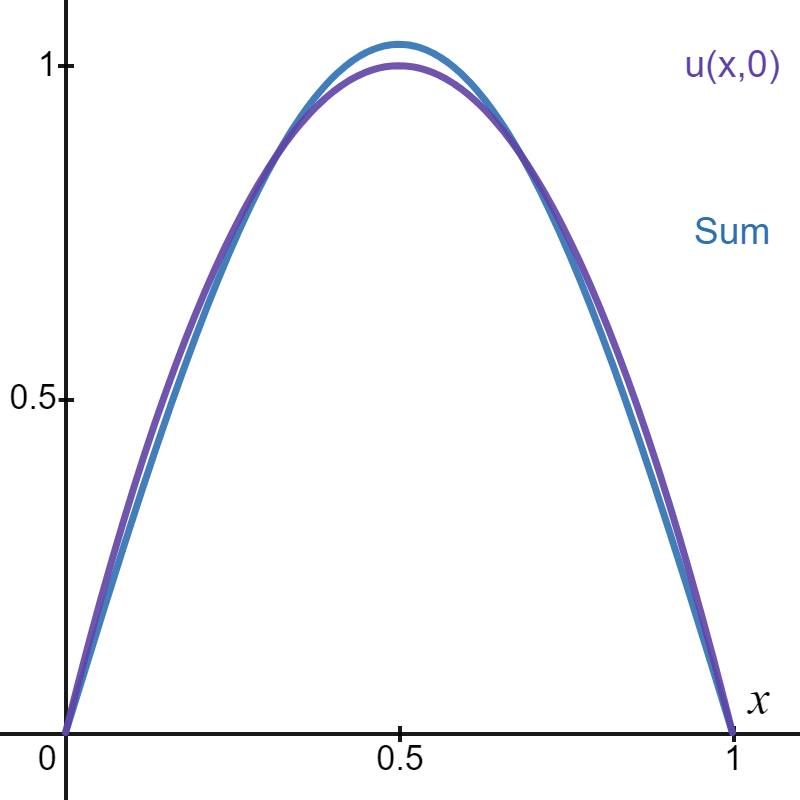
\includegraphics[width=\textwidth]{figures/sum_n1.png}
        \caption{Plotting both $u(x,0)$ and the sum up to $N=1$.}
    \end{subfigure}
    \hfill
    \begin{subfigure}[b]{0.3\textwidth}
        \centering
        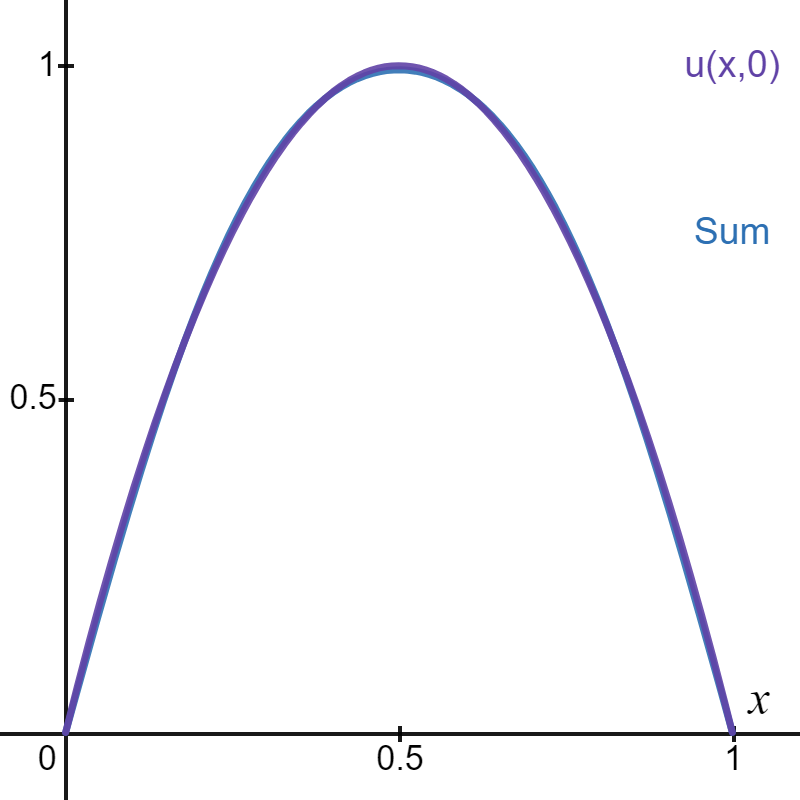
\includegraphics[width=\textwidth]{figures/sum_n4.png}
        \caption{Plotting both $u(x,0)$ and the sum up to $N=4$.}
    \end{subfigure}
    \hfill
    \begin{subfigure}[b]{0.3\textwidth}
        \centering
        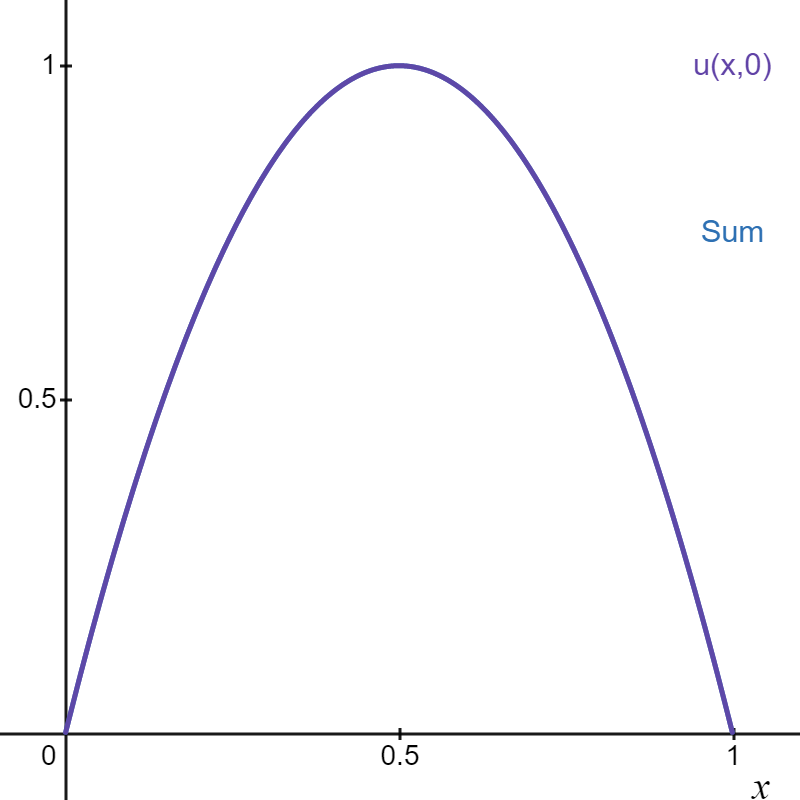
\includegraphics[width=\textwidth]{figures/sum_n50.png}
        \caption{Plotting both $u(x,0)$ and the sum up to $N=50$.}
    \end{subfigure}
    \end{figure}

\item It is true we can do this for any physically meaningful (finite energy) initial condition. Basically, if the initial condition had infinite area under the curve, things could go awry. 
\end{enumerate}
\end{solution}
\vspace*{1cm}
\textcolor{red}{
\noindent \textbf{Rubric:}
\begin{enumerate}[(a)]
    \item \textbf{(1 pt.)} Brief and reasonable explanation.
    \item \textbf{(1 pt.)} Brief and reasonable explanation.
    \item \textbf{(1 pt.)} Graph on the proper domain of original function or the approximation. \textbf{(1 pt.)} Both graphs put up simultaneously and the number of terms used shows the convergence of the series to the intended function.
	\textbf{(1 pt.)} Reasonable discussion on why this would or would not work. Answer does not need to match mine.
\end{enumerate}
}

\newpage
\begin{problem}
\textbf{(12 pt.)} Previously we studied the time-independent Schr\"odinger equation. Now, we can take a look at the time-dependent version given by
\[
\left( H - i\hbar \frac{\partial}{\partial t} \right) \Psi(x,t) = 0,
\]
where $H$ is the Hamiltonian operator.  

Consider the situation for the free particle in the 1-dimensional box of length $1$ so that $V(x)=0$ and $\Psi(0,t)=0=\Psi(1,t)$. Hence, the problem
\[
\begin{cases}
\left( -\frac{\hbar}{2m} \frac{\partial ^2}{\partial x^2} - i\hbar \frac{\partial}{\partial t} \right) \Psi(x,t) = 0 & \textrm{in the region $\Omega = [0,1]$}\\
\Psi(0,t)=0=\Psi(1,t), & \textrm{as boundary conditions}.
\end{cases}
\]
Note that for each $n$ we have a normalized state
\[
\psi_n(x,t) = \sqrt{2} e^{-i \frac{E_n}{\hbar} t} \sin(n \pi x)
\]
where 
\[
E_n = \frac{n^2 \pi^2 \hbar^2}{2m}
\]
is the energy eigenvalue.
\begin{enumerate}[(a)]
    \item \textbf{(1 pt.)} Argue that a linear combination (superpostion) of states is a solution by noting that the operator
	\[
	\mathcal{L} = -\frac{\hbar}{2m} \frac{\partial ^2}{\partial x^2} - i\hbar \frac{\partial}{\partial t}
	\]
	is linear. \emph{Hint: think about kernels and subspaces.}
    \item \textbf{(2 pt.)} For a single state $\psi_n(x,t)$, show that the probability amplitude
    \[
\left|\psi_n(x,t)\right|^2
    \]
    is independent of $t$. This shows that the states $\psi_n$ are \emph{stationary} since their probability amplitude does not depend on time.
	\item \textbf{(3 pt.)} When a particle is in superposition, then the probability amplitude can change over time. Consider the superposition wavefunction
	\[
	\Psi = \frac{1}{\sqrt{2}} \left( \psi_1 + \psi_2 \right).
	\]
	Show that the probability amplitude can be written as
	\[
	|\Psi|^2 = 2 \cos(\omega_R t)\sin(\pi x)\sin(2\pi x)+ \sin(\pi x)^2 +\sin(2\pi x)^2
	\]
	and determine $\omega_R$ in terms of the energy eigenvalues. Note that $\omega_R$ is called the \emph{Rabi frequency} and this occurs in two-state systems.
	\item \textbf{(1 pt.)} Quickly verify that the total probability amplitude for the superposition wavefunction $\Psi$ is 1. \emph{Hint: please just use the fact that the states are orthonormal!}
	\item \textbf{(2 pt.)} Make an animation of the probability amplitude on the given domain $\Omega$ on Desmos. (For credit: show your Desmos code or show a few slices of the probability amplitude over time.)
	\item \textbf{(1 pt.)} Can you interpret your answer in part (d) as motion of the particle? Explain.
	\item \textbf{(2 pt.)} Given an initial wave function $\Psi(x,0)$, how can you determine $\Psi(x,t)$? \emph{Hint: consider what we discuss in Problem 1. Can you take an infinite linear combination of states? If so, how do you determine the coefficients?}
\end{enumerate}
\end{problem}
\begin{solution}~
\begin{enumerate}[(a)]
\item By definition of $\mathcal{L}$ given here, the time-dependent Schr\"odinger equation is given by
\[
\mathcal{L} \Psi = 0
\]
and thus $\Psi \in \ker \mathcal{L}$. Since the kernel of a transformation is always a subspace and a subspace is closed under linear combinations, any linear combination of solutions is also a solution.

\begin{remark}
The reason why an infinite sum of solutions is a solution is because $\mathcal{L}$ is also continuous (which I have \emph{not} defined!)
\end{remark}

\item We have
\begin{align*}
|\psi_n|^2 = \psi_n^* \psi_n  &= \sqrt{2} e^{i \frac{E_n}{\hbar} t} \sin(n \pi x) \cdot \sqrt{2} e^{-i \frac{E_n}{\hbar} t} \sin(n \pi x)\\
&=2 e^{i \frac{E_n}{\hbar} t}e^{-i \frac{E_n}{\hbar} t} \sin^2(n\pi x)\\
&= 2 \sin^2(n \pi x),
\end{align*}
hence the time component disappears and the probability amplitude is stationary.

\item We have
\begin{align*}
	|\Psi|^2 &= \frac{1}{2} \left( |\psi_1|^2 + \psi_1^* \psi_2 + \psi_2^* \psi_1 + |\psi_2|^2 \right)\\
&= \frac{1}{2} \left(e^{i\frac{E_1-E_2}{\hbar}t} + e^{i\frac{E_2-E_1}{\hbar}t}\right) \sin(\pi x)\sin(2 \pi x)+ \sin(\pi x)^2 +\sin(2\pi x)^2 && \textrm{used result from (b)}\\
&= 2 \cos\left( \frac{E_2-E_1}{\hbar} t\right)\sin(\pi x)\sin(2\pi x)+ \sin(\pi x)^2 +\sin(2\pi x)^2.
\end{align*}
Hence, the Rabi frequency is $\omega_R= \frac{E_2-E_1}{\hbar}$.

\item We have
\begin{align*}
	\innprod{\Psi}{\Psi} &= \innprod{\frac{1}{\sqrt{2}(\psi_1 + \psi_2)}}{\frac{1}{\sqrt{2}(\psi_1 + \psi_2)}}\\
	&= \frac{1}{2}\underbrace{\innprod{\psi_1}{\psi_1}}_{=\delta_{11} = 1} +  \underbrace{\innprod{\psi_1}{\psi_2}}_{=\delta_{12} = 0} + \frac{1}{2}\underbrace{\innprod{\psi_2}{\psi_2}}_{=\delta_{22} = 1}\\
	&= \frac{1}{2} + \frac{1}{2} = 1.
\end{align*}

\item Here is a figure that shows the evolution over time.
\begin{figure}[H]
	\centering
	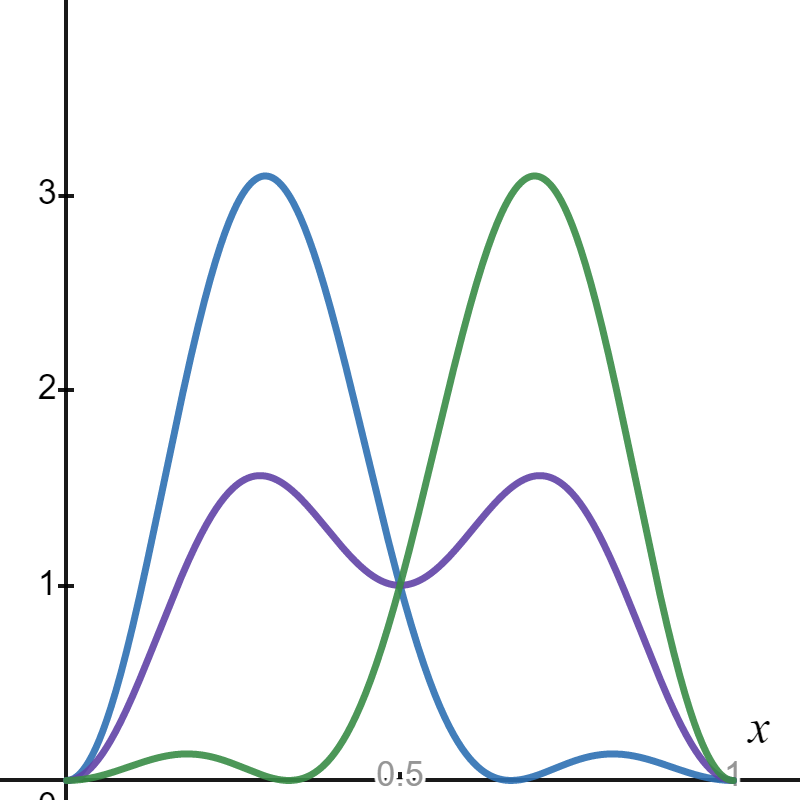
\includegraphics[width=0.5\textwidth]{figures/time_dependent_superposition.png}
	\caption{I chose to set $\hbar=m=1$ to plot this. The blue curve represents time $t_0=0$, the purple curve is midway through the oscillation by choosing $t_1= \frac{1}{6\pi}$, and the green curve is when the probability has ``swapped sides'' and this happens when $t_2=\frac{2}{6\pi}$.}
\end{figure}

\item I would say that this is close to motion. The most likely position to find the particle does change over time, so if you were to make repeated measurements of a system like this it would appear that the particle oscillates on average.

\item Given $\Psi(x,0)$ we can compute the projection onto the basis $\psi_n(x)$ by
\[
\Psi(x,0) = \sum_{n=1}^\infty \innprod{\Psi(x,0)}{\psi_n(x)} \psi_n(x)
\]
and to make this a function of time we can just write
\[
\Psi(x,t) = \sum_{n=1}^\infty \innprod{\Psi(x,0)}{\psi_n(x)} \psi_n(x,t).
\]
\end{enumerate}
\end{solution}
\vspace*{1cm}
\textcolor{red}{
\noindent \textbf{Rubric:}
\begin{enumerate}[(a)]
    \item \textbf{(1 pt.)} Mention that kernel is a subspace and you can take linear combinations in a subspace.
    \item \textbf{(1 pt.)} Final answer does not have a $t$ variable. \textbf{(1 pt.)} Valid work to get to final answer.
    \item \textbf{(1 pt.)} Correct form of final answer. \textbf{(1 pt.)} Valid work to get to final answer. \textbf{(1 pt.)} Correct Rabi frequency.
	\item \textbf{(1 pt.)} Valid work and final answer. 
	\item \textbf{(1 pt.)} Nice looking graph on the proper domain. \textbf{(1 pt.)} Slices in time that show how the probability amplitude changes.
	\item \textbf{(1 pt.)} A reasonable discussion on what they see in the graph. Answer does not have to match mine.
	\item \textbf{(1 pt.)} An thorough explanation or valid work to show how you can get the coefficients for $\Psi(x,0)$ for a series. \textbf{(1 pt.)} A throrough explanation or valid work to show how you can make this depend on time.
\end{enumerate}
}


\newpage
\begin{problem}
\textbf{(7 pt.)} Maxwell's equations are given as
\begin{align*}
\grad \cdot \vecfieldB &= 0  & \grad \cdot \vecfieldE &= \frac{\rho}{\epsilon_0}\\
\grad \times \vecfieldB -\mu_0 \epsilon_0\frac{\partial \vecfieldE}{\partial t}&=\mu_0 \vecfieldJ & \grad \times \vecfieldE + \frac{\partial \vecfieldB}{\partial t} &= \zerovec
\end{align*}
\begin{enumerate}[(a)]
    \item \textbf{(2 pt.)} Look up each of the terms in the equations above and describe them.
    \item \textbf{(2 pt.)} Describe what each equation is saying and why these are PDEs.
    \item \textbf{(2 pt.)} In the absence of all charges we will have $\vecfieldJ=\zerovec$ and $\rho=0$.  Using that and the following two facts
    \[
    \veclaplace \vecfieldV = \grad (\grad \cdot \vecfieldV) - \grad \times (\grad \times \vecfieldV) \qquad \textrm{and} \qquad \grad \times \frac{\partial \vecfieldV}{\partial t} = \frac{\partial}{\partial t} (\grad \times \vecfieldV),
    \]
    derive the vector wave equations for light
    \[
    \left( - \veclaplace + \mu_0 \epsilon_0 \frac{\partial^2 }{\partial t^2}\right) \vecfieldE = \zerovec
    \]
    and
    \[
    \left( - \veclaplace + \mu_0 \epsilon_0 \frac{\partial^2 }{\partial t^2}\right) \vecfieldB = \zerovec
    \]
    \item \textbf{(1 pt.)} From the equations you derived, determine the wave speed of light in the vacuum, $c_0$.
\end{enumerate}
\end{problem}
\begin{solution}~
\begin{enumerate}[(a)]
    \item From top left to bottom right, we have names for the equations.  They are:
    \begin{itemize}
        \item Gauss's law for magnetism: $\grad \cdot \vecfieldB = 0$.
        \item Gauss's law: $\grad \cdot \vecfieldE = \frac{\rho}{\epsilon_0}$.
        \item Amp\`ere's circuital law: $\grad \times \vecfieldB -\mu_0 \epsilon_0\frac{\partial \vecfieldE}{\partial t}=\mu_0 \vecfieldJ$.
        \item Faraday's law of induction: $\grad \times \vecfieldE + \frac{\partial \vecfieldB}{\partial t} = \zerovec$.
    \end{itemize}
    
    In the above equations we have a few terms that we should define and describe.  First, there are the fields, $\vecfieldE$ and $\vecfieldB$ which are the electric and magnetic fields respectively.  Both are functions of space and time, so we could put $\vecfieldE(x,y,z,t)$ and $\vecfieldB(x,y,z,t)$ if we wanted to be a bit more transparent.  Both of these fields cause forces on charged particles and arise from the single electromagnetic field that permeates all of space.  Indeed, the fields themselves can also arise from charged particles as well.  They can also take on different values depending on how the charges are placed or whether or not they are moving.
    
    We refer to the static distribution of charge with the variable $\rho$ which physically represents the charge density.  In principle, this charge density (per unit volume) can depend on both space and time and we could put $\rho(x,y,z,t)$ to again be fully transparent.  There may also be a current density (per unit area) present in space, which we represent by $\vecfieldJ$. Again, this is a function that can change over space and time and we could put $\vecfieldJ(x,y,z,t)$.  The electric and magnetic fields become unified into the single electromagnetic field when we start to think of $\rho$ and $\vecfieldJ$ as describing an analogous quantity. One can realize this by noting that moving charges are what generate a current.  If two observers are to view the same configuration of charges and currents from different perspectives (different reference frames) they may disagree on the values for $\vecfieldE$ and $\vecfieldB$.  However, if you properly transform space and time between their perspectives, you will see that this difference just has to do with their differences in relative motion.  This sparked the idea of Einstein and other physicists and mathematicians (like Lorentz) to develop \emph{special relativity}.  Under special relativity, we see that these two fields $\vecfieldE$ and $\vecfieldB$ are just portions of the electromagnetic field that depend on your relative motion.
    
    Finally, we can take a look at the constants $\epsilon_0$ and $\mu_0$ which appear.  In general, $\epsilon$ describes the permittivity of a substance.  That is, how freely the electric field $\vecfieldE$ can pass through a given substance.  The subscript $0$ pertaining to $\epsilon_0$ states that this is the permittivity of free space (i.e., the permittivity of the vacuum).  In this sense, even the vacuum has some notion of resisting how the electric field can pass through it. On the flip side, $\mu$ describes the permeability of a substance.  It is the magnetic analog to $\epsilon$. So, in this case, $\mu_0$ represents the permeability of the vacuum.  Roughly speaking, $\mu$ is describing how easily a substance allows the magnetic field to pass through it. One should be a bit careful here.  We are actually finding that we may need to think about these quantities in different ways as we learn more.  So, this point of view may be a bit defunct in some ways.
    
    \item The above equations are indeed PDEs.  For each, we are intending to find vector fields that satisfy conditions.  In fact, each equation is coupled to one another.  Specifically, what this means is that we require the vector field $\vecfieldE$ and $\vecfieldB$ to simultaneously solve all of the above equations. We take $\rho$ and $\vecfieldJ$ to be external to these equations in that these are values we supply in order to determine the induced fields $\vecfieldE$ and $\vecfieldB$.  
    
    In this sense, these are PDEs of vector fields while all the previous examples we had considered were PDEs of scalar fields.  One may then refer to these equations as vector PDEs and the others as scalar PDEs.  
    
    Lastly, it may be illuminating to see that if we supply no charge density $\rho$ and no current density $\vecfieldJ$, that the equations above still provide \underline{nontrivial} solutions! That is, the vector fields aren't just constants.  We will see this in the next part.
    
    If we remove all current density by taking $\vecfieldJ$ to be zero and we let $\rho(x,y,z)$ not depend on time, then we arrive at the vacuum electrostatic equations
    \begin{align*}
        \grad \times \vecfieldE = \zerovec \qquad \textrm{and} \qquad \grad \cdot \vecfieldE = \frac{\rho}{\epsilon_0}.
    \end{align*}
    Here, we can see that $\vecfieldE$ is conservative since its curl is zero.  Indeed, that means there exists a potential function $\phi(x,y,z)$ such that $\grad \phi = \vecfieldE$.  This potential is called the \emph{electrostatic potential} or the \emph{voltage}.  Thus, the equations simply reduce to finding a scalar field $\phi$ such that
    \[
    \Delta \phi = \frac{\rho}{\epsilon_0},
    \]
    which is the Poisson equation.  Once again, we arrive back at an equation we have seen in other contexts. Note that this means we actually only define $\phi$ up to a constant! Typically, we choose to let this constant be zero.  One may call this \emph{gauge fixing}.
    
    Analogously, we can force $\rho$ to be zero and let $\vecfieldJ(x,y,z)$ not depend on time and we arrive at the realm of the vacuum magnetostatic equations given by
    \[
        \grad \cdot \vecfieldB = 0 \qquad \textrm{and} \qquad \grad \times \vecfieldB = \mu_0 \vecfieldJ.
    \]
    Note that when we are working in $\R^3$, if we have $\grad \cdot \vecfieldB=0$, it means that $\vecfieldB = \grad \times \vecfieldA$ where we refer to the vector field $\vecfieldA$ as the \emph{vector potential} for the vector field $\vecfieldB$.  This is analogous to having a scalar potential when a vector field is curl free. By the Helmholtz decomposition of vector fields, we know that $\vecfieldA$ can be written as a part that is curl free plus a part that is divergence free. Thus, if we choose to let $\grad \cdot \vecfieldA=0$, we can still satisfy $\grad \times \vecfieldA = \vecfieldB$ and by doing this we have
    \[
    \grad \left(\grad \cdot \vecfieldA\right) - \grad \times \left(\grad \times \vecfieldA\right)= \veclaplace \vecfieldA = \vecfieldJ.
    \]
    However, the divergence of $\vecfieldA$ being zero implies that we must have
    \[
    \veclaplace \vecfieldA = \vecfieldJ,
    \]
    which is the vector form of the Laplace equation.  The choice of forcing the extra condition
    \[
    \grad \cdot \vecfieldA=0,
    \]
    fixes what we refer to as the \emph{Coulomb gauge}.  One may also notice that the idenity
    \[
    \grad \cdot \left( \grad \times \vecfieldV \right) = 0,
    \]
    means that we must have $\grad \cdot \vecfieldJ=0$.  So, we can only find magnetostatic vector fields when we have a source/sink free current.
    
    \item Now, let us fix $\rho=0$ and $\vecfieldJ=\zerovec$.  Then, we can take the curl of Faraday's law yields
        \begin{align*}
            \grad \times \left(\grad \times \vecfieldE +  \frac{\partial \vecfieldB}{\partial t} \right) &=\zerovec\\
            \implies ~ \grad \times \left(\grad \times \vecfieldE\right) + \grad \times \left(\frac{\partial \vecfieldB}{\partial t} \right)&=\zerovec \\
            \implies ~ \grad \left( \grad \cdot \vecfieldE\right)-\veclaplace \vecfieldE + \frac{\partial}{\partial t} \left( \grad \times \vecfieldB\right)&=\zerovec\\
            \implies ~ -\veclaplace \vecfieldE +  \frac{\partial}{\partial t} \left(\mu_0 \epsilon_0 \frac{\partial \vecfieldE}{\partial t}\right) &= \zerovec\\
            \implies ~ \left( - \veclaplace + \mu_0 \epsilon_0 \frac{\partial^2 }{\partial t^2}\right) \vecfieldE &= \zerovec,
        \end{align*}
        which is our intended equation.  Likewise, we can take the curl of Amp\`ere's law to get
    \begin{align*}
        \grad \times \left(\grad \times \vecfieldB - \mu_0 \epsilon_0 \frac{\partial \vecfieldE}{\partial t} \right) &=\zerovec\\
        \implies ~ \grad \times \left(\grad \times \vecfieldB\right) - \grad \times \left(\mu_0 \epsilon_0\frac{\partial \vecfieldE}{\partial t} \right)&=\zerovec \\
        \implies ~ \grad \left( \grad \cdot \vecfieldB\right)-\veclaplace \vecfieldB - \mu_0\epsilon_0\frac{\partial}{\partial t} \left( \grad \times \vecfieldE\right)&=\zerovec\\
        \implies ~ -\veclaplace \vecfieldB - \mu_0 \epsilon_0 \frac{\partial}{\partial t} \left(-\frac{\partial \vecfieldB}{\partial t}\right) &= \zerovec\\
        \implies ~ \left( - \veclaplace + \mu_0 \epsilon_0 \frac{\partial^2 }{\partial t^2}\right) \vecfieldB &= \zerovec,
    \end{align*}
    which is the other intended equation. These are both the vector wave equations for the electromagnetic field. Otherwise known as light.
    
    \item The wavespeed in the wave equation is typically written as $c$ and appears as
    \[
    \left( - \veclaplace + \frac{1}{c^2} \frac{\partial^2 }{\partial t^2}\right).
    \]
    Hence, the wave speed here is
    \[
    c_0 = \frac{1}{\sqrt{\mu_0\epsilon_0}} = 2.998 \cdot 10^8 m/s,
    \]
    which is the speed of light in the vacuum.
\end{enumerate}
\end{solution}
\vspace*{1cm}
\textcolor{red}{
\noindent \textbf{Rubric:}
\begin{enumerate}[(a)]
    \item \textbf{(1 pt.)} Each term is mentioned. \textbf{(1 pt.)} Each term is given some kind of physical interpretation.
    \item \textbf{(1 pt.)} Mention that we are solving for $\vecfieldE$ and $\vecfieldB$ given $\vecfieldJ$ and $\rho$. \textbf{(1 pt.)} Explanation for why they are PDEs.
    \item \textbf{(1 pt.)} Correct work for both equations. \textbf{(1 pt.)} Correct final answers.
	\item \textbf{(1 pt.)} Correct algebraic value for $c_0 = \frac{1}{\sqrt{\mu_0 \epsilon_0}}$. Students do not have to look up the numerical value, but they really should have!
\end{enumerate}
}

\end{document}